\begin{frame}{Who? - Lecturers}
	%Melanie Bianca Sigl
	\begin{columns}
		\begin{column}{0.8\textwidth}
			\begin{itemize}
				\item \textbf{Melanie Bianca Sigl, M.Sc.:}
				      \begin{itemize}
					      \item External Ph.D. candidate
					      \item PRODATO Integration Technology GmbH
					      \item E-Mail: \href{mailto:melanie.sigl@fau.de}{melanie.sigl@fau.de}
					      \item Website: \url{https://www.cs6.tf.fau.eu/person/melanie-sigl/}
				      \end{itemize}
			\end{itemize}
		\end{column}
		\begin{column}{0.2\textwidth}
			\begin{center}
				\includegraphics[width=0.5\textwidth]{img/melanie_b_sigl.jpg}
			\end{center}
		\end{column}
	\end{columns}

	%Dominik Probst
	\begin{columns}
		\begin{column}{0.8\textwidth}
			\begin{itemize}
				\item \textbf{Dominik Probst, M.Sc.:}
				      \begin{itemize}
					      % Following the guidelines for our business cards without "Chair of"
					      \item Ph.D. candidate
					      \item Computer Science 6 (Data Management)
					      \item E-Mail: \href{mailto:dominik.probst@fau.de}{dominik.probst@fau.de}
					      \item Website: \url{https://www.cs6.tf.fau.de/person/dominik-probst/}
				      \end{itemize}
			\end{itemize}
		\end{column}
		\begin{column}{0.2\textwidth}
			\begin{center}
				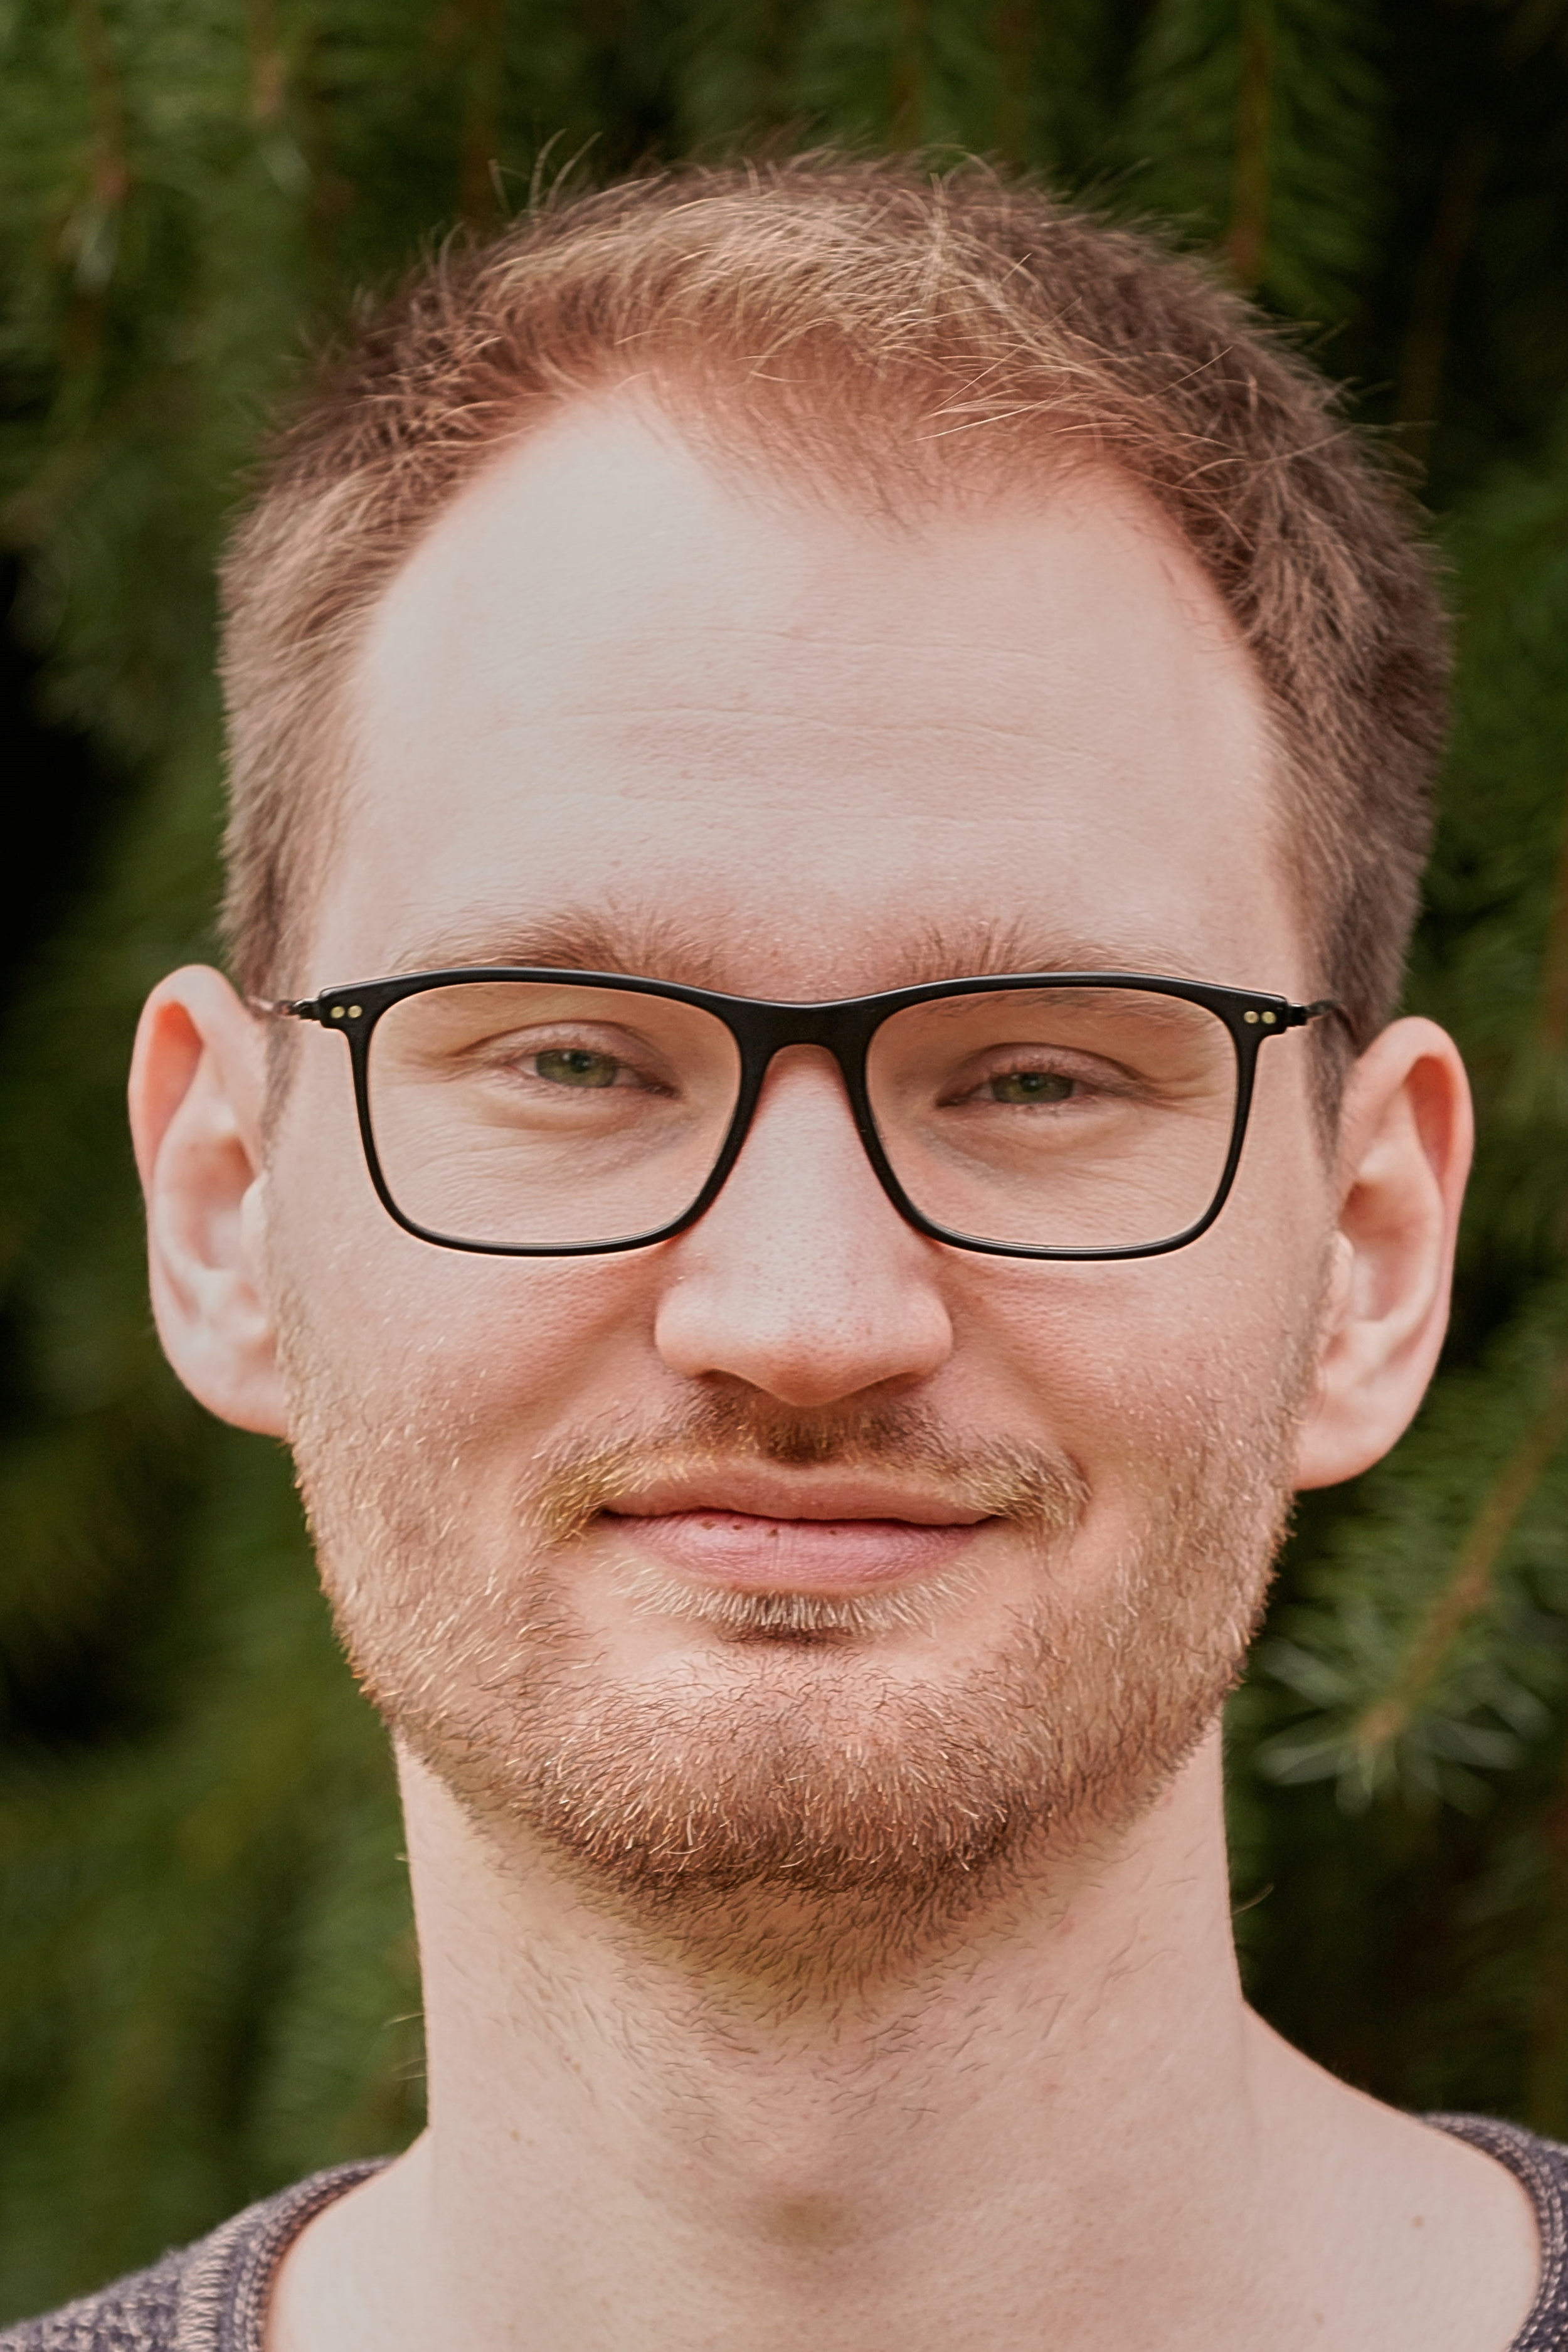
\includegraphics[width=0.5\textwidth]{img/dominik_probst.jpg}
			\end{center}
		\end{column}
	\end{columns}
\end{frame}

\begin{frame}{For whom? - Courses of study}
	% Study programs
	\begin{itemize}
		\item \textbf{Knowledge Discovery in Databases with exercise (KDDmUe)} - 5 ECTS
		      \begin{itemize}
			      \item B.Sc. Data Science
			      \item M.Sc. Computer Science
			      \item {\color{gray} Possibly other courses of study (clarify with your examination office)}
		      \end{itemize}
		\item \textbf{Knowledge Discovery in Databases (KDD)} - 2.5 ECTS
		      \begin{itemize}
			      \item M.Sc. Information- and Communication Technology
			      \item M.Sc. Medical Engineering
		      \end{itemize}
	\end{itemize}

	\begin{alertblock}{Important: KDDmUe replaces KDDTAS in B.Sc. Data Science!}
		The module KDDTAS, which is listed in the examination regulations of B.Sc. Data Science, is no longer offered by us. The module KDDmUe is the replacement for it and is recognized by us accordingly.
	\end{alertblock}
\end{frame}

\begin{frame}{For whom? - Prerequisites}
	%Prerequisites
	\begin{itemize}
		\item \textbf{Mandatory requirements:}
		      \begin{itemize}
			      \item Successful completion of the module \glqq Konzeptionelle Modellierung\grqq
		      \end{itemize}
		\item \textbf{Useful prerequisites:}
		      \begin{itemize}
			      \item Successful completion of the module \glqq Implementierung von Datenbanksystemen\grqq
			      \item Experience with:
			            \begin{itemize}
				            \item Python
				            \item Jupyter Notebooks
				            \item Numpy
				            \item Pandas
				            \item \ldots
			            \end{itemize}
		      \end{itemize}
	\end{itemize}

\end{frame}


\begin{frame}{What? - Goal and topics}
	% Goal of the lecture
	\begin{itemize}
		\item \textbf{Goal of the module:}
		      \begin{itemize}
			      \item Introduce you to the principles of data mining. \\
			            $\Rightarrow$ This is the core of knowledge discovery in databases
		      \end{itemize}
		\item \textbf{Topics in the lecture:}
		      \vspace*{-1\multicolsep}
		      \begin{multicols}{2}
			      \begin{enumerate}
				      \item Introduction {\color{gray} - D. Probst}
				      \item Data {\color{gray} - M. B. Sigl}
				      \item Preprocessing {\color{gray} - D. Probst}
				      \item Data Warehousing {\color{gray} - M. B. Sigl}
				      \item Mining Frequent Patterns {\color{gray} - D. Probst}
				      \item Classification {\color{gray} - M. B. Sigl}
				      \item Cluster Analysis {\color{gray} - D. Probst}
				      \item Outlier Analysis {\color{gray} - M. B. Sigl}
				      \item {\color{gray}Guest lecture by Friedrich-Claus Grüber (Siemens Energy)}
			      \end{enumerate}
		      \end{multicols}
		      \vspace*{-1\multicolsep}
		\item \textbf{Topics in the exercise:}
		      \vspace*{-1\multicolsep}
		      \begin{multicols}{2}
			      \begin{enumerate}
				      \item Introduction to Python
				      \item Data
				      \item Frequent Patterns
				      \item Classification
				      \item Clustering
				      \item Outlier
			      \end{enumerate}
		      \end{multicols}
		      \
	\end{itemize}
\end{frame}

\begin{frame}{What? - Exam}
	% Exam
	\begin{itemize}
		\item \textbf{Knowledge Discovery in Databases with exercise (KDDmUe)} - Written
		      \begin{itemize}
			      \item Duration: 90 minutes
			      \item Questions about the lecture and the exercise
			      \item {\color{gray} Language: English}
		      \end{itemize}
		\item \textbf{Knowledge Discovery in Databases (KDD)} - Oral
		      \begin{itemize}
			      \item Duration: 30 minutes
			      \item Questions about the lecture
			      \item {\color{gray} Language: English or German}
		      \end{itemize}
	\end{itemize}
	\begin{alertblock}{Important: Don't forget to register!}
		Without exception, we can only examine participants who have also registered for this with the examination office. Please pay attention to the information of the examination office when the registration takes place in this semester.
	\end{alertblock}
\end{frame}

\begin{frame}{What? - Literature}
	% Literature
	\begin{itemize}
		\item \textbf{The lecture is based on the following book:}
		      \begin{itemize}
			      \item \fullcite{han2011}
			      \item Copies are available at the Science and Technology Branch Library (TNZB).
			      \item Slides have been downloaded from \href{http://hanj.cs.illinois.edu/}{Jiawei Han's web server} and modified.
			      \item Previous iterations of the modified slides were created by Prof. Dr.-Ing. Klaus Meyer-Wegener and Luciano Melodia.
		      \end{itemize}
		\item \textbf{Also interesting and related textbooks are:}
		      \begin{itemize}
			      \item \fullcite{geron2017}
			      \item \fullcite{du2010}
			      \item \fullcite{witten2016}
			      \item \ldots
		      \end{itemize}
	\end{itemize}
\end{frame}

\begin{frame}{When? - Dates}
	% Dates
	\begin{itemize}
		\item \textbf{Lecture} - Start in Calendar Week 17 (Today)
		      \begin{itemize}
			      \item Monday, 10:15 - 11:45 (Online via Zoom) \\
			            {\color{gray}Lecturers: M. B. Sigl and D. Probst}
		      \end{itemize}
		\item \textbf{Exercises} - Start in Calendar Week 18
		      \begin{itemize}
			      \item Wednesday, 14:15 - 15:45 (H8) \\
			            {\color{gray}Tutor: D. Probst}
			      \item Friday, 16:15 - 17:45 (Online via Zoom) \\
			            {\color{gray}Tutors: M. B. Sigl and D. Probst}
		      \end{itemize}
	\end{itemize}

	\begin{block}{Registration for the exercises}
		In order to ensure the most even distribution to the exercises, registration for the exercises is required. This is possible starting at April 25 (18:00) in our StudOn course.
	\end{block}
\end{frame}

\begin{frame}{When? - Schedule}
	% Schedule
	\begin{itemize}
		\item \textbf{Current schedule} - Subject to Change
	\end{itemize}
	\begin{center}
		\resizebox{0.8\textwidth}{!}{
			\begin{tabular}{|l|l|l|}
				\hline
				\textbf{Calendar Week} & \textbf{Lecture}                                    & \textbf{Exercise}                                               \\ \hline
				17                     & Prologue + Introduction                             &                                                                 \\ \hline
				18                     & Data                                                & Introduction to Pandas \& scikit-learn {\color{gray}(optional)} \\ \hline
				19                     & \multirow{2}{*}{Preprocessing}                      & \multirow{3}{*}{Data analysis \& data preprocessing}            \\ \cline{1-1}
				20                     &                                                     &                                                                 \\ \cline{1-2}
				21                     & {\color{gray}Guest lecture (Siemens Energy) +} OLAP &                                                                 \\ \hline
				22                     & \multirow{2}{*}{Frequent Pattern}                   & \multirow{2}{*}{Frequent Pattern}                               \\ \cline{1-1}
				23                     &                                                     &                                                                 \\ \hline
				24                     & \multirow{2}{*}{Classification}                     & \multirow{2}{*}{Classification}                                 \\ \cline{1-1}
				25                     &                                                     &                                                                 \\ \hline
				26                     & \multirow{2}{*}{Cluster Analysis}                   & \multirow{2}{*}{Clustering}                                     \\ \cline{1-1}
				27                     &                                                     &                                                                 \\ \hline
				28                     & \multirow{2}{*}{Outlier Analysis}                   & Outlier                                                         \\ \cline{1-1} \cline{3-3}
				29                     &                                                     &                                                                 \\ \hline
				30                     & Current Research at CS6 + Exam Q\&A                 &                                                                 \\ \hline
			\end{tabular}}
	\end{center}
\end{frame}

\begin{frame}{Where? - StudOn}
	% StudOn
	\begin{columns}
		\begin{column}{0.7\textwidth}
			\begin{itemize}
				\item \textbf{StudOn:}
				      \begin{itemize}
					      \item Register at: \url{https://www.studon.fau.de/crs4353407_join.html}
					      \item Main source for resources. E.g.:
					            \begin{itemize}
						            \item Zoom access data
						            \item Lecture slides
						            \item Exercise sheets
						            \item \ldots
					            \end{itemize}
					      \item Membership required to receive important updates on KDD by mail
					      \item Questions should be asked here (StudOn Forum)

				      \end{itemize}
			\end{itemize}
		\end{column}
		\begin{column}{0.3\textwidth}
			\begin{center}
				\qrcode{https://www.studon.fau.de/crs4353407_join.html}
			\end{center}
		\end{column}
	\end{columns}

\end{frame}


\begin{frame}{Where? - GitHub}
	% GitHub
	\begin{columns}
		\begin{column}{0.7\textwidth}
			\begin{itemize}
				\item \textbf{GitHub:}
				      \begin{itemize}
					      \item Public repository at: \url{https://github.com/FAU-CS6/KDD}
					      \item Version control of our ressources. E.g.:
					            \begin{itemize}
						            \item Lecture slides
						            \item Exercise sheets
						            \item \ldots
					            \end{itemize}
				      \end{itemize}
			\end{itemize}
		\end{column}
		\begin{column}{0.3\textwidth}
			\begin{center}
				\qrcode{https://github.com/FAU-CS6/KDD}
			\end{center}
		\end{column}
	\end{columns}
	\vspace{5mm}
	\begin{block}{Error corrections}
		We know that there will never be error-free slides or practice sheets. However, you can help us get as close as possible: If you find an error in our documents, you can correct it on your own in our GitHub repository and ask us to merge it into the offical documents via pull request.
	\end{block}

\end{frame}
